\chapter{VIC-IV Video Interface Controller}
\label{cha:viciv}

\section{Features}
The VIC-IV is a fourth generation Video Interface Controller developed
especially for the MEGA65, and featuring very good backwards compatibility
with the VIC-II that was used in the C64, and the VIC-III that
was used in the C65.  The VIC-IV can be programmed as though it were either
of those predecessor systems.  In addition it supports a number of new
features. It is easy to mix older VIC-II/III features with the new VIC-IV
features, making it easy to transition from the VIC-II or VIC-III to the VIC-IV,
just as the VIC-III made it easy to transition from the VIC-II.  Some of the new
features and enhancements of the VIC-IV include:

\begin{itemize}
\item {\bf Direct access to 384KB RAM} (up from 16KB/64KB with the VIC-II and 128KB
  with the VIC-III).
\item Support for {\bf 32KB of 8-bit Colour/Attribute RAM} (up from 2KB on the VIC-III), to
  support very large screens.
\item {\bf HDTV 720$\times$576 / 800$\times$600 native resolution} at both 50Hz and 60Hz for {\bf PAL and NTSC}, with {\bf VGA and digital video} output.
\item {\bf 81MHz pixel clock} (up from $\sim$ 8MHz with the VIC-II/III), which enables a wide range of new features.
\item New 16-colour (16$\times$8 pixels per character cell) and 256-colour (8$\times$8 pixels per character cell) {\bf full-colour text modes}.
\item Support for up to {\bf 8,192 unique characters in a character set}.
\item {\bf Four 256-colour palette banks} (versus the VIC-III's single palette bank), each supporting {\bf 23-bit colour depth} (versus the VIC-III's 12-bit colour depth), and which can be rapidly alternated to create even more colourful graphics than is possible with the VIC-III.
\item Screen, bitmap, colour and character data can be positioned at any {\bf address with byte-level granularity} (compared with fixed 1KB -- 16KB boundaries with the VIC-II/III)
\item {\bf Virtual screen dimensioning}, which combined with byte-level data position granularity provides effective {\bf hardware support for scrolling and panning in both X and Y directions}.
\item {\bf New sprite modes}: Bitplane modification, {\bf full-colour} (15 foreground colours + transparency) and tiled modes, allowing a wide variety of new and exciting sprite-based effects
  \item The ability to stack sprites in a bit-planar manner to produce {\bf sprites with up to 256 colours}.
\item Sprites can use 64 bits of data per raster line, allowing {\bf sprites to be 64 pixels wide} when using VIC-II/III mono/multi-colour mode, or 16 pixels wide when using the new VIC-IV full-colour sprite mode.
\item {\bf Sprite tile mode}, which allows a sprite to be repeated horizontally across an entire raster line, allowing sprites to be used to create  animated backgrounds in a memory-efficient manner.
  \item Sprites can be configured to use a {\bf separate 256-colour palette} to that used to draw other text and graphics, allowing for a more colourful display.
  \item {\bf Super-extended attribute mode} which uses two screen RAM bytes and two colour RAM bytes per character mode, which supports a wide variety of new features including {\bf alpha-blending/anti-aliasing}, {\bf hardware kerning/variable-width characters}, hardware horizontal/vertical flipping, alternate palette selection and other powerful features that make it easy to create highly dynamic and colourful displays.
  \item {\bf Raster-Rewrite Buffer} which allows {\bf hardware-generated pseudo-sprites}, similar to ``bobs'' on Amiga\texttrademark{} computers, but with the advantage that they are rendered in the display pipeline, and thus do not need to be un-drawn and redrawn to animate them.
    \item {\bf Multiple 8-bit colour play-fields} are also possible using the Raster-Rewrite Buffer.

      In short, the VIC-IV is a powerful evolution of the VIC-II/III, while retaining the character and distinctiveness of the VIC-series of
      video controllers.

      For a full description of the additional registers that the VIC-IV provides, as well as documentation of the legacy VIC-II and VIC-III registers, refer to the corresponding sections of this appendix. The remainder of the appendix will focus on describing the capabilities and use of many of the VIC-IV's new features.
\end{itemize}

\section{VIC-II/III/IV Register Access Control}
Because the new features of the VIC-IV are all extensions to the existing VIC-II/III designs, there is no concept of having to select the mode in which the VIC-IV will operate: It is always in VIC-IV mode. However, for backwards compatibility with software, the many additional registers of the VIC-IV can be hidden, so that it appears to be either a VIC-II or VIC-III. This is done in the same manner that the VIC-III uses to hide its new features from legacy VIC-II software.

 The mechanism is the VIC-III write-only KEY register (\$D02F, 53295 decimal).  The VIC-III by default conceals its new features until a ``knock'' sequence is performed.  This consists of writing two special values one after the other to \$D02F.  The following table summarises the knock sequences supported by the VIC-IV, and indicates which are VIC-IV specific, and which are supported by the VIC-III:

\setlength{\tabcolsep}{3pt}
\begin{longtable}{|L{2.4cm}|L{2.4cm}|L{3.5cm}|L{2cm}|}
\hline
{\bf{First Value Hex (Decimal)}} & {\bf{Second Value Hex (Decimal)}} & {\bf{Effect}} & {\bf{VIC-IV Specific? }} \\
\hline
\endfirsthead
\multicolumn{3}{l@{}}{\ldots continued}\\
\hline
{\bf{First Value Hex (Decimal)}} & {\bf{Second Value Hex (Decimal)}} & {\bf{Effect}} & {\bf{VIC-IV Specific? }} \\
\endhead
\multicolumn{3}{l@{}}{continued \ldots}\\
 \endfoot
 \hline
\endlastfoot
\small \$00 (0) & \small \$00 (0) & Only VIC-II registers visible (all VIC-III and VIC-IV new registers are hidden) & No \\
 \hline
\small \$A5 (165) & \small \$96 (150) & VIC-III new registers visible & No \\
 \hline
\small \$47 (71) & \small \$53 (83) & Both VIC-III and VIC-IV new registers visible & Yes \\
 \hline
\small \$45 (69)  & \small \$54 (84) & No VIC-II/III/IV registers visible. 45E100 Ethernet controller buffers are visible instead & Yes \\
 \hline
   \end{longtable}


 \subsection{Detecting VIC-II/III/IV}

 Detecting which generation of the VIC-II/III/IV a machine is fitted with can be important for programs that support only particular generations, or that wish to vary their graphical display based on the capabilities of the machine.  While there are many possibilities for this, the following is a simple and effective method.  It relies on the fact that the VIC-III and VIC-IV do not repeat the VIC-II registers throughout the I/O address space.  Thus while \$D000 and \$D100 are synonymous when a VIC-II is present (or a VIC-III/IV is hiding their additional registers), this is not the case when a VIC-III or VIC-IV is making all of its registers visible.  Therefore presence of a VIC-III/IV can be determined by testing whether these two locations are aliases for the same register, or represent separate registers.
 The detection sequence consists of using the KEY register to attempt to make either VIC-IV or VIC-III additional registers visible. If either succeeds, then we can assume that the corresponding generation of VIC is installed. As the VIC-IV supports the VIC-III KEY knocks, we must first test for the presence of a VIC-IV.  Also, we assume that the MEGA65 starts in VIC-IV mode, even when running C65 BASIC.  Thus the test can be done in BASIC from either C64 or C65-mode as follows:

\begin{screenoutput}
0 REM IN C65-MODE WE CANNOT SAFELY WRITE TO $D02F, SO WE TEST A DIFFERENT WAY
10 IF PEEK($D018) AND 32 THEN GOTO 65
20 POKE $D000,1:POKE $D02F,71:POKE $D02F,83
30 POKE $D000+256,0:IF PEEK($D000)=1 THEN PRINT"VIC-IV PRESENT":END
40 POKE $D000,1:POKE $D02F,165:POKE $D02F,150
50 POKE $D000+256,0:IF PEEK($D000)=1 THEN PRINT"VIC-III PRESENT":END
60 PRINT "VIC-II PRESENT":END
65 REM WE ASSUME WE HAVE A C65 HERE
70 V1=PEEK($D050):V2=PEEK($D050):V3=PEEK($D050)
80 IF V1<>V2 OR V1<>V3 OR V2<>V3 THEN PRINT "VIC-IV PRESENT":END
90 GOTO 40
\end{screenoutput}

Line 10 of this program checks whether the screen is a multiple of 2KB.
As the screen on the C64 is located at 1KB, this test will fail, and execution
will continue to line 20.  Line 20 writes 1 to one of the VIC-II sprite position
registers, 53248, before writing the MEGA65 knock to the key register, 53295.
Line 30 writes to 53248 + 256, which on the C64 is a mirror of 53248, but on a
MEGA65 with VIC-IV I/O enabled will be one of the red palette registers.
After writing to 53248 + 256, the program checks if the register at 53248 has
been modified by the write to 53248 + 256.  If it has, then the two addresses
point to the same register.  This will happen on either a C64 or C65, but not on
a computer with a VIC-IV.  Thus if 53248 has not changed, we report that we have detected a VIC-IV.
If writing to 53248 + 256 did change the value in register 53248, then we proceed
to line 40, which writes to 53248 again, and this time writes the VIC-III knock to
the key register.  Line 50 is like line 30, but as it appears after a VIC-III knock,
it allows the detection of a VIC-III.  Finally, if neither a VIC-IV nor VIC-III
is detected, we conclude that only a VIC-II must be present.

As the MEGA65 is the only C64-class computer that is fitted with a
VIC-IV, this can be used as a {\em de facto} test for the presence of
a MEGA65 computer. Detection of a VIC-III can be similarity assumed to
indicate the presence of a C65.

\section{Video Output Formats, Timing and Compatibility}

\subsection{Integrated Marvellous Digital Hookup\texttrademark{} (IMDH\texttrademark{})
  Digital Video Output}
  \index{Integrated Marvellous Digital Hookup\texttrademark}
  \index{IMDH\texttrademark}

The MEGA65 features VGA analog video output and Integrated Marvellous
Digital Hookup\texttrademark{} (IMDH\texttrademark{}). This is different
to existing common digital video standards in several key points:

\begin{enumerate}
  \item We didn't invent a new connector for it: We instead used the
    most common digital video connector already in use.  So your
    existing cables should work fine!
  \item We didn't make it purposely incompatible with any existing
    digital video standard. So your existing TVs and monitors should
    work fine!
  \item We don't engage in highway-robbery for other vendors to use
    the IMDH\texttrademark{} digital video standard, by trying to
    charge them \$10,000 every year, just for the permission to be
    able to sell a single device. This means that the MEGA65 is
    cheaper for you!
  \item The IMDH\texttrademark{} standard does not allow
    content-protection or other sovereignty eroding flim-flam. If you
    produced the video, you can do whatever you like with it!
\end{enumerate}

\subsubsection{Connecting to Naughty Proprietary Digital Video
  Standards}
\index{digital video}

There are digital video standards that are completely backwards compared
with IMDH\texttrademark. Fortunately because of IMDH\texttrademark's
open approach to interoperability, these should, in most cases,
function with the MEGA65 without difficulty.  Simply find a video
cable fits the IMDH\texttrademark{} connector on the back of your MEGA65, and connect
it to your MEGA65 and a TV, Monitor or Projector that has the same
connector.

However, regrettably, not all manufacturers
have submitted their devices for IMDH\texttrademark{} compliance testing with the
MEGA65 team. This means that some TVs and Monitors are,
unfortunately, not IMDH\texttrademark{} compliant.  Thus while most TVs and Monitors
will work with the MEGA65, you might find that you need to try a
couple to get a satisfactory result.  If you do find a monitor that
doesn't work with the MEGA65, please let us know, and also report the
problem to the Monitor vendor, recommending that they submit their
devices for IMDH\texttrademark{} compliance testing.

The VIC-IV was designed for use in the MEGA65 and related systems, including the MEGAphone family of portable devices.
The VIC-IV supports both VGA and digital video output, using the
non-proprietary IMDH\texttrademark{} interface.
It also supports parallel digital video output suitable for driving LCD display
panels.  Considerable care has been taken to create a common video front-end that supports these three output modes.

For simplicity and accuracy of frame timing for legacy software, the video format is normally based on the HDTV PAL and NTSC 720$\times$576/480 (576p and 480p) modes using a 27MHz output pixel clock.  This is ideal for digital video and LCD display panels. However not all VGA displays support
these modes, especially 720$\times$576 at 50Hz.

In terms of VIC-II and VIC-III backwards compatibility, this display format has several effects that do not cause problems for most programs, but can cause some differences in behaviour:

\begin{enumerate}
\item Because the VIC-IV display is progressive rather than interlaced, two physical raster lines are produced for each logical VIC-II or VIC-III raster line.  This means that there are either 63 or 65 cycles per logical double raster, rather than per physical 576p/480p physical raster. This can cause some minor visual artefacts, when programs make assumptions about where on a horizontal line the VIC is drawing when, for example, the border or screen colour is changed.
\item The VIC-IV does not follow the behaviour of the VIC-III, which allowed changes in video modes, e.g., between text and bitmap mode, on characters.  Nor does it follow the VIC-II's policy of having such changes take effect immediately.  Instead, the VIC-IV applies changes at the start of each raster line.  This can cause some minor artefacts.
\item The VIC-IV uses a single-raster rendering buffer which is populated using the VIC-IV's internal 81MHz pixel clock, before being displayed using the 27MHz output pixel clock.  This means that a raster lines display content tends to be rendered much earlier in a raster line than on either the VIC-II or VIC-III.  This can cause some artefacts with displays, particularly in demos that rely on specific behaviour of the VIC-II at particular cycles in a raster line, for example for effects such as VSP or FLI.  At present, such effects are unlikely to display correctly on the current revision of the VIC-IV.  Improved support for these features is planned for a future revision of the VIC-IV.
  \item The 1280$\times$200 and 1280$\times$400 display modes of the VIC-III are not currently supported, as they cannot be meaningfully displayed on any modern monitor, and no software is known to support or use this feature.
\end{enumerate}

\subsection{Frame Timing}

Frame timing is designed to match that of the 6502 + VIC-II combination of the C64.  Both PAL and NTSC timing is supported, and the number of cycles per logical raster line, the number of raster lines per frame, and the number of cycles per frame are all adjusted accordingly.  To achieve this, the VIC-IV ordinarily uses HDTV 576p 50Hz (PAL) and 480p 60Hz (NTSC) video modes, with timing tweaked to be as close as possible to double-scan PAL and NTSC composite TV modes as used by the VIC-II.

The VIC-IV produces timing impulses at approximately 1MHz which are used by the 45GS02 processor, so that the correct effective frequency is provided when operating at the 1MHz, 2MHz and 3.5MHz C64, C128 and C65 compatibility modes.  This allows the single machine to switch between accurate PAL and NTSC CPU timing, as well as video modes. The exact frequency varies between PAL and NTSC modes, to mimic the behaviour of PAL versus NTSC C64, C128 and C65 processor and video timing.

The PAL frame is constructed from 624 physical raster lines, consisting of 864 pixel clock ticks. The pixel clock is 27MHz, which is 1/3 the VIC-IV pixel clock.  The visible frame is 720$\times$576 pixels, the entirety of which can be used in VIC-IV mode. In VIC-II and VIC-III modes, the border area reduces the usable size to 640$\times$400 pixels.  In VIC-II mode and VIC-III 200H modes, the display is double scanned, with two 31.5 micro-second physical rasters corresponding to a single 63 micro-second VIC-II-style raster line.  Thus each frame consists of 312 VIC-II raster lines of 63 micro-seconds each, exactly matching that of a PAL C64.

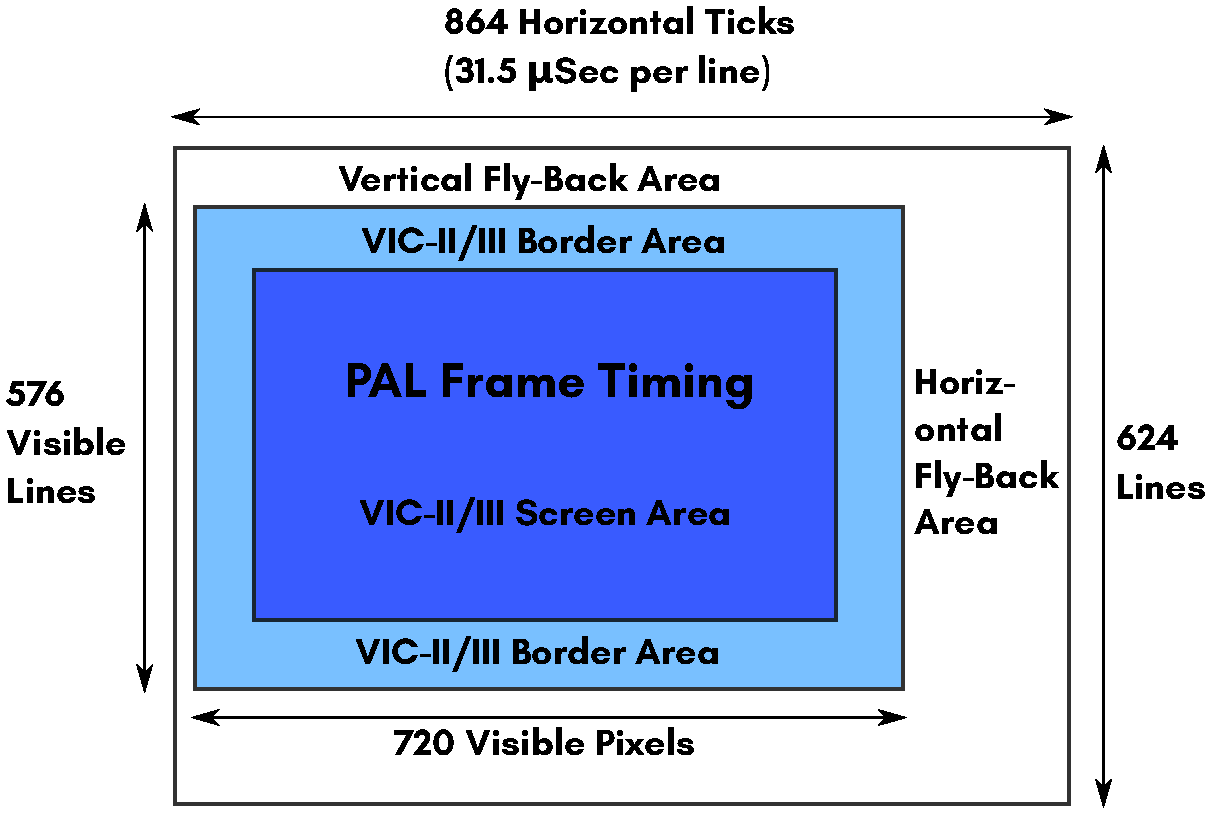
\includegraphics[width=\linewidth]{images/illustrations/VIC-IV-PAL-Frame.pdf}

The NTSC frame is constructed from 526 physical raster lines, consisting of 858 pixel clock ticks. The pixel clock is 27MHz, which is 1/3 the VIC-IV pixel clock.  The visible frame is 720$\times$480 pixels, the entirety of which can be used in VIC-IV mode. In VIC-II and VIC-III modes, the border area reduces the usable size to 640$\times$400 pixels.  In VIC-II mode and VIC-III 200H modes, the display is double scanned, with two 32 micro-second physical rasters corresponding to a single 64 micro-second VIC-II-style raster line.  Thus each frame consists of 263 VIC-II raster lines of 64 micro-seconds each, matching the most common C64 NTSC video timing.

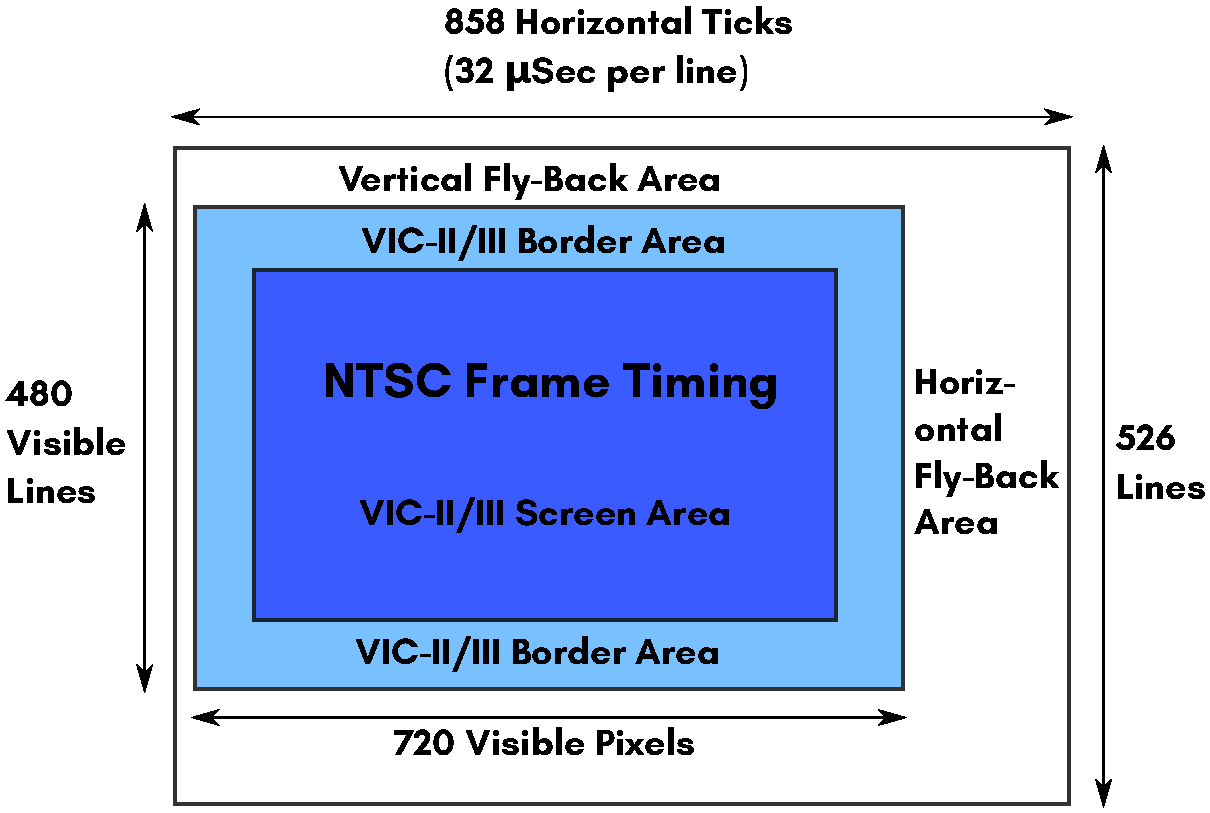
\includegraphics[width=\linewidth]{images/illustrations/VIC-IV-NTSC-Frame.pdf}

As these HDTV video modes are not supported by all VGA monitors, a compatibility mode is included that provides a 640$\times$480 VGA-style mode. However, as the pixel clock of the MEGA65 is fixed at 27MHz, this mode runs at 63Hz.  Nonetheless, this should work on the vast majority of VGA monitors.  There should be no problem with the PAL / NTSC modes when using the digital video output of the MEGA65 with the vast majority of IMDH\texttrademark-enabled monitors and TVs.

To determine whether the MEGA65 is operating in PAL or NTSC, you can enter the Freeze Menu, which displays the current video mode, or from a program you can check the PALNTSC signal (bit 7 of \$D06F, 53359 decimal). If this bit is set, then the machine is operating in NTSC mode, and clear if operating in PAL mode. This bit can be modified to change between the modes, e.g.:

\begin{tcolorbox}[colback=black,coltext=white]
\verbatimfont{\codefont}
\begin{verbatim}
10 REM ENABLE C65+MEGA65 I/O
20 IF PEEK($D018)<32 THEN POKE $D02F,ASC("G"):POKE $D02F,ASC("S")
30 REM CHECK NTSC BIT
40 NTSC=PEEK($D06F) AND 128
50 REM DISPLAY STATE AND ASK FOR TOGGLE
60 PRINT"MEGA65 IS IN ";:IF NTSC THEN PRINT"NTSC MODE":ELSE PRINT"PAL MODE"
70 INPUT"SWITCH MODES (Y/N)? ",A$
80 REM TOGGLE NTSC BIT
90 IF A$="Y" THEN POKE $D06F,PEEK($D06F) XOR 128:ELSE END
100 REM DISPLAY NEW STATE
110 NTSC=PEEK($D06F) AND 128
120 PRINT"MEGA65 IS IN ";:IF NTSC THEN PRINT"NTSC MODE":ELSE PRINT"PAL MODE"
\end{verbatim}
\end{tcolorbox}

\subsubsection{Physical and Logical Rasters}

Physical rasters per frame refers to the number of actual raster lines in the PAL or
NTSC Enhanced Definition TV (EDTV) video modes used by the MEGA65.  Logical Rasters refers to the number of VIC-II-style rasters per frame.
Each logical raster consists of two physical rasters per line, since EDTV modes are double-scan modes compared with the original PAL and NTSC
Standard Definition TV modes used by the C64. The frame parameters of the VIC-IV for PAL and NTSC are as follows:

\setlength{\tabcolsep}{3pt}
\begin{longtable}{|L{2cm}|L{2.5cm}|L{2.5cm}|L{2.5cm}|}
\hline
{\bf{Standard}} & {\bf{Cycles per Raster}} & {\bf{Physical Rasters per Frame}} & {\bf{Logical Rasters per Frame}}  \\
\hline
\endfirsthead
\multicolumn{3}{l@{}}{\ldots continued}\\
\hline
{\bf{Standard}} & {\bf{Cycles per Raster}} & {\bf{Physical Rasters per Frame}} & {\bf{Logical Rasters per Frame}}  \\
\endhead
\multicolumn{3}{l@{}}{continued \ldots}\\
\endfoot
\hline
\endlastfoot
	\small PAL & 63 & 626 & 312  \\
	\small NTSC & 65 & 526 & 263  \\
\end{longtable}

The result is that the frames on the VIC-IV consist of exactly the same
 number of $\sim$ 1MHz CPU cycles as on the VIC-II exactly.

\subsubsection{Bad Lines}

The VIC-IV does not natively incur any ``bad lines'', because the VIC-IV has its own dedicated memory busses to the main memory
and colour RAM of the MEGA65.  This means that both the processor and VIC-IV can access the memory at the same time, unlike on the
C64 or C65, where they are alternated.

However, to improve compatibility, the VIC-IV signals when a ``bad line'' would have occurred on the VIC-II.  The 45GS02 processor
of the MEGA65 accepts these bad line signals, and pauses the CPU for 40 clock cycles, except if the processor is running
at full speed, in which case they are ignored.  This improves the timing compatibility with the VIC-II considerably.  However,
the timing is not exact, because the current revision of the 45GS02 pauses for exactly 40 cycles, instead of 40 -- 43 cycles,
depending on the instruction being executed at the time. Also, the VIC-IV and 45GS02 do not currently pause for sprite fetches.


The bad line emulation is controlled by bit 0 of \$D710: setting this bit enables bad line emulation, and clearing it prevents
any bad line from stealing time from the processor.


\section{Memory Interface}

The VIC-IV supports up to 16MB of direct access RAM for video data, however at present, all existing models provide only 384KB of addressable RAM.
In MEGA65 systems, the second block of 128KB of RAM (spanning from 128KB-256KB in the memory map) is typically used to hold a C65-compatible ROM,
leaving 256KB of RAM available to the user. If software is written to avoid the need to use C65 ROM routines, then the entire 384KB of RAM can be used by the program.

All MEGA65 models presently support 32KB of colour RAM, however there are plans for the latest R3 board to support 64KB of colour RAM (or possibly even 128KB).

The VIC-IV supports all legacy VIC-II and VIC-III methods for accessing this RAM, including the VIC-II's use of 16KB banks, and the VIC-III's Display Address Translator (DAT).  This additional memory can be used for character and bitmap displays, as well as for sprites.  However, the VIC-III bitplane modes remain limited to using only the first 128KB of RAM, as the VIC-IV does not enhance the bitplane mode.

\subsection{Relocating Screen Memory}

To use the additional memory for screen RAM, the screen RAM start address can be adjusted to any location in memory with byte-level granularity by setting the SCRNPTR registers (\$D060 -- \$D063, 53344 -- 53347 decimal).  For example, to set the screen memory to address 12345:

\begin{tcolorbox}[colback=black,coltext=white]
\verbatimfont{\codefont}
\begin{verbatim}
REM ENABLE C65+MEGA65 I/O
IF PEEK($D018)<32 THEN POKE $D02F,ASC("G"):POKE $D02F,ASC("S")
POKE $D060,$45:POKE $D061,$23:POKE $D062,$1
\end{verbatim}
\end{tcolorbox}

\subsection{Relocating Character Generator Data}

The location of the character generator data can also be set with byte-level precision via the CHARPTR registers at \$D068 -- \$D06A (53352 -- 53354 decimal). As usual, the first of these registers holds the lowest-order byte, and the last the highest-order byte. The three bytes allow for placement of character data anywhere in the first 16MB of RAM. For systems with less than 16MB of RAM accessible by the VIC-IV, the upper address bits should be zero.

For example, to indicate that character generator data should be sourced beginning at \$41200 (266752 decimal), the following
could be used.  Note that the AND binary operator only works with arguments between 0 and 65,535. Therefore we first
subtract 4$\times$65,536 = 262,144 from the address (the 4 is determined by calculating INT(266752/65536) ), before we use the AND operator to compute the lower part of the address:

\begin{tcolorbox}[colback=black,coltext=white]
\verbatimfont{\codefont}
\begin{verbatim}
REM ENABLE C65+MEGA65 I/O
IF PEEK($D018)<32 THEN POKE $D02F,ASC("G"):POKE $D02F,ASC("S")
REM HEX $41200 IS EASILY DIVIDED IN ITS 3 BYTES $00, $12, $4
REM BUT YOU CAN ALSO USE MATH TO EXTRACT THE PARTS
POKE $D060,(266752-INT(266752/65536)*$10000) AND 255
POKE $D061,INT((266752-INT(266752/65536)*65536)/256)
POKE $D062,INT(266752/65536)
\end{verbatim}
\end{tcolorbox}


\subsection{Relocating Colour / Attribute RAM}

The area of colour RAM being used can be similarly set using the COLPTR registers (\$D064 -- \$D065, 53348 -- 53349 decimal). That is, the value is an offset from the start of the colour / attribute RAM.  This is because, like on the C64, the colour / attribute RAM of the MEGA65 is a separate memory component, with its own dedicated connection to the VIC-IV.  By default, the COLPTRs are set to zero, which replicates the behaviour of the VIC-II/III.  To set the display to use the colour / attribute RAM beginning at offset \$4000, one could use something like:

\begin{tcolorbox}[colback=black,coltext=white]
\verbatimfont{\codefont}
\begin{verbatim}
REM ENABLE C65+MEGA65 I/O
IF PEEK($D018)<32 THEN POKE $D02F,ASC("G"):POKE $D02F,ASC("S")
REM SET COLPTR TO $4000, SPLITS INTO $00 LSB and $40 MSB
POKE $D064,$00
POKE $D065,$40
\end{verbatim}
\end{tcolorbox}

\subsection{Relocating Sprite Pointers and Images}

The location of the sprite pointers can also be moved, and sprites can be made to have their data anywhere in first 4MB of memory.
This is accomplished by first setting the location of the sprite pointers by setting the SPRPTRADR registers (\$D06C -- \$D06E, 53356 -- 53358 decimal, but note that only the bottom 7 bits of \$D06E are used, as the highest bit is used for the SPRPTR16 signal).  This allows the list of
eight sprite pointers to be moved from the end of screen RAM to an arbitrary location in the first 8MB of RAM.  To allow sprites themselves
to be located anywhere in the first 4MB of RAM, the SPRPTR16 bit in \$D06E must be set. In this mode, two bytes are used to indicate the
location of each sprite, instead of one. That is, the list of sprite pointers will be 16 bytes long, instead of 8 bytes long as on the VIC-II/III.  When SPRPTR16 is enabled, the location of the sprite pointers should always be set explicitly via the SPRPTRADR registers.
For example, to position the sprite pointers at location 800 -- 815, you could use something like the following code. Note that a little gymnastics is required to keep the SPRPTR16 bit unchanged, and also to work around the AND binary operator not working with values greater than 65535:

\begin{tcolorbox}[colback=black,coltext=white]
\verbatimfont{\codefont}
\begin{verbatim}
REM ENABLE C65+MEGA65 I/O
IF PEEK($D018)<32 THEN POKE $D02F,ASC("G"):POKE $D02F,ASC("S")
POKE $D06C,(800-INT(800/65536)*65536) AND 255
POKE $D06D,INT(800/256) AND 255
POKE $D06E,(PEEK($D06E) AND 128)+INT(800/65536)
\end{verbatim}
\end{tcolorbox}

The location of each sprite image remains a multiple of 64 bytes, thus allowing for up to 65,536 unique sprite images
to be used at any point in time, if the system is equipped with sufficient RAM (4MB or more).  In this mode, the VIC-II 16KB banking is ignored, and the location of sprite data is simply 64 $\times$ the pointer value.  For example, to have the data for a sprite at \$C000 (49152 decimal), this would be sprite location 768, because 49152 divided by 64 = 768.  We then need to split 768 into high and low bytes, to set the two pointer bytes: 768 = 256$\times$3, with remainder 0, so this would require the two sprite pointer bytes to be 0 (low byte, which comes first) and 3 (high byte).  Thus if the sprite pointers were located at \$7F8 (2040 decimal), setting the first sprite to sprite image 768 could be done with something like:

\begin{screenoutput}
POKE 2040,768-256*INT(768/256)
POKE 2041,INT(768/256)
\end{screenoutput}

\section{Hot Registers}

Because of the availability of precise vernier registers to set a wide
range of video parameters directly, \$D011 (53265 decimal), \$D016 (53270 decimal) and other VIC-II and
VIC-III video mode registers are implemented as virtual registers:
by default, writing to any of these results in computed consistent values being
applied to all of the relevant vernier registers.  This means that
writing to any of these virtual registers will reset the video mode.
Thus some care has to be taken when using new VIC-IV features to not
touch any of the ``hot'' VIC-II and VIC-III registers.

The ``hot'' registers to be careful with are:

\$D011, \$D016, \$D018, \$D031 (53265, 53270, 53272 and 53297 decimal) and the VIC-II bank bits of \$DD00 (56576 decimal).

If you write to any of those, various VIC-IV registers will need to be re-written
with the values you wish to maintain.

This ``hot'' register behaviour is intended primarily for legacy software.
It can be disabled by clearing the HOTREG signal (bit 7 of \$D05D, 53341 decimal).

\section{New Modes}

\subsection{Why the new VIC-IV modes are Character and Bitmap modes, not Bitplane modes}

The new VIC-IV video modes are derived from the VIC-II character and bitmap modes, rather than the VIC-III
bitplane modes. This decision was based on several realities of programming a memory-constrained 8-bit home computer:

\begin{enumerate}
\item Bitplanes require that the same amount of memory is given to each area on screen, regardless of whether it
is showing empty space, or complex graphics. There is no way with bitplanes to reuse content from within an image in
another part of the image.  However, most C64 games use highly repetitive displays, with common elements appearing in various
places on the screen, of which Boulder Dash and Super Giana Sisters would be good examples.

\item Bitplanes also make it difficult to update a display, because every pixel is unique, in that there is no way to make a change,
for example to the animation in an onscreen element, and have it take effect in all places at the same time. The diamond
animations in Boulder Dash are a good example of this problem.  The requirement to modify multiple separate bytes in each
bitplane create an increased computational burden, which is why there were calls for the Amiga AAA chip-set to include so-called
``chunky'' modes, rather than just bitplane based modes.  While the Display Address Translator (DAT) and DMAgic of the C65 provide some
relief to this problem, the relief is only partial.

\item Scrolling using the C65 bitplanes requires copying the entire bitplane, as the hardware support for smooth scrolling does not
extend to changing the bitplane source address in a fine manner.  Even using the DMAgic to assist, scrolling a 320$\times$200 256-colour
display requires 128,000 clock cycles in the best case (reading and writing 320$\times$200 = 64000 bytes). At 3.5MHz on the C65 this
would require about 36 milli-seconds, or about 2 complete video frames.  Thus for smooth scrolling of such a display, a double
buffered arrangement would be required, which would consume 128,000 of the 131,072 bytes of memory.

In contrast, the well known character modes of the VIC-II are widely used in games, due to their ability to allow a small amount
of screen memory to select which 8$\times$8 block of pixels to display, allowing very rapid scrolling, reduced memory consumption, and
effective hardware acceleration of animation of common elements.  Thus the focus of improvements in the VIC-IV has been on
character mode.  As bitmap mode on the VIC-II is effectively a special case of character mode, with implied character numbers, it
comes along free for the ride on the VIC-IV, and will only be mentioned in the context of a very few bitmap-mode specific
improvements that were trivial to make, and it thus seemed foolish to not implement, in case they find use.

\end{enumerate}

\subsection{Displaying more than 256 unique characters via
"Super-Extended Attribute Mode"}

The primary innovation is the addition of the Super-Extended Attribute Mode. The VIC-II already uses 12 bits per character: Each 8$\times$8
cell is defined by 12 bits of data: 8 bits of screen RAM data, by
default from \$0400 -- \$07E7 (1024 -- 2023 decimal), indicating which
characters to show, and 4 bits of colour data from the 1K nibble colour
RAM at \$D800 -- \$DBFF (55296 -- 56319 decimal). The VIC-III of the
C65 uses 16 bits, as the colour RAM is now 8 bits, instead of 4, with
the extra 4 bits of colour RAM being used to support attributes (blink,
bold, underline and reverse video).  It is recommended to revise how
this works, before reading the following. A good introduction to the
VIC-II text mode can be found in many places.
% For example, \ref{vicii-cheaper-by-the-dozen}. <- undefined
Super-Extended Attribute mode doubles the number of bits per character used from the VIC-III’s 16, to 32: Two bytes of screen RAM and two bytes of
colour/attribute RAM.

Super-Extended Attribute Mode is enabled by setting bit 0 in \$D054
(53332 decimal). Remember to first enable VIC-IV mode, to make this
register accessible. When this bit is set, two bytes are used for each
of the screen memory and colour RAM for each character shown on the
display. Thus, in contrast to the 12 bits of information that the C64
uses per character, and the 16 bits that the VIC-III uses, the VIC-IV
has 32 bits of information.  How those 32 bits are used varies slightly
among the particular modes.  The default is as follows:

\setlength{\tabcolsep}{3pt}
\begin{longtable}{|L{3cm}|L{8cm}|}
\hline
{\bf{Bit(s)}} & {\bf{Function}}  \\
\hline
\endfirsthead
\multicolumn{2}{l@{}}{\ldots continued}\\
\hline
{\bf{Bit(s)}} & {\bf{Function}}  \\
\endhead
\multicolumn{2}{l@{}}{continued \ldots}\\
\endfoot
\hline
\endlastfoot
\small Screen RAM byte 0 & {\small Lower 8 bits of character number, the same as the VIC-II and VIC-III }\\
\small Screen RAM byte 1, bits 0 - 4 & {\small Upper 5 bits of character number, allowing addressing of 8,192 unique characters }\\
\small Screen RAM byte 1, bits 5 -- 7 & {\small Trim pixels from right-hand side of character (bits 0 -- 2) {\em or} Set character data Y offset if GOTOX set set (bits 0 -- 2) }\\
\small Colour RAM byte 0, bit 7 & {\small Vertically flip the character {\em or} enable transparency for subsequent characters if GOTOX is set }\\
\small Colour RAM byte 0, bit 6 & {\small Horizontally flip the character }\\
\small Colour RAM byte 0, bit 5 & {\small Alpha blend mode (leave 0, discussed later) }\\
\small Colour RAM byte 0, bit 4 & {\small GOTO X (allows repositioning of characters along a raster via the Raster-Rewrite Buffer, discussed later), must be set to 0 for displaying characters }\\
\small Colour RAM byte 0, bits 3 & {\small If set, Full-Colour characters use 4 bits per pixel and are 16 pixels wide (less any right-hand side trim bits), instead of using 8 bits per pixel. When using 8 bits per pixels, the characters are the normal 8 pixels wide  }\\
\small Colour RAM byte 0, bits 2 & {\small Trim pixels from right-hand side of character (bit 3) {\em or} Set character data Y offset if GOTOX set set (bit 3) }\\
\small Colour RAM byte 0, bits 0 -- 1 & {\small Number of pixels to trim from top or bottom of character }\\
\small Colour RAM byte 1, bits 0 -- 3 & {\small Low 4 bits of colour of character }\\
\small Colour RAM byte 1, bits 4 -- 7 & {\small Upper 4 bits of colour of character (if VIC-II multi-colour mode is enabled) }\\
\small Colour RAM byte 1, bit 4 & {\small Hardware blink of character (if VIC-III extended attributes are enabled) }\\
\small Colour RAM byte 1, bit 5 & {\small Hardware reverse video enable of character (if VIC-III extended attributes are enabled)* }\\
\small Colour RAM byte 1, bit 6 & {\small Hardware bold attribute of character (if VIC-III extended attributes are enabled)* }\\
\small Colour RAM byte 1, bit 7 & {\small Hardware underlining of character (if VIC-III extended attributes are enabled) }\\
\end{longtable}

* Enabling BOLD and REVERSE attributes at the same time on the MEGA65 selects an alternate palette, effectively allowing 512 colours on screen, but each 8$\times$8 character can use colours only from one 256 colour palette.

If the GOTOX bit is set, some of the fields have different meanings:

\setlength{\tabcolsep}{3pt}
\begin{longtable}{|L{3cm}|L{8cm}|}
\hline
{\bf{Bit(s)}} & {\bf{Function}}  \\
\hline
\endfirsthead
\multicolumn{2}{l@{}}{\ldots continued}\\
\hline
{\bf{Bit(s)}} & {\bf{Function}}  \\
\endhead
\multicolumn{2}{l@{}}{continued \ldots}\\
\endfoot
\hline
\endlastfoot
\small Screen RAM byte 0 & {\small Lower 8 bits of new X position to start drawing the next character, relative to the start of character drawing.  Setting to 0 causes the next character to be drawn over the top of the left-most character. }\\
\small Screen RAM byte 1, bits 0 - 1 & {\small Upper 2 bits of new X position }\\
\small Screen RAM byte 1, bits 3 - 4 & {\small RESERVED, set to 0 }\\
\small Screen RAM byte 1, bits 5 - 7 & {\small FCM Character data offset: Characters display normally when set to zero. When non-zero, 8 $\times$ the value is added to the character address. With careful planning, this can be used to smoothly vertically scroll multiple layers of RRB content.  }\\
\small Colour RAM byte 0, bit 4 - 5 & {\small RESERVED, set to 0 }\\
\small Colour RAM byte 0, bits 6 & {\small If set, the following characters will be rendered as background, allowing sprites to appear in front of them, even when sprites are set to background. }\\
\small Colour RAM byte 0, bit 7 & {\small If set, then background/transparent pixels will not be drawn, allowing layering }\\
\small Colour RAM byte 0, bit 4 & {\small GOTO X, set to 1 }\\
\small Colour RAM byte 0, bits 3 & {\small ROWMASK. If set, then the pixel row mask is used to determine which pixel rows of the following characters should be rendered. This can be used to vertically scroll characters using the Raster-Rewrite Buffer, by drawing each character twice, once shifted down on the screen line on which it appears, and a second time, shifted up in the following screen line, and masked so that only the pixel rows belonging to the scrolled character are displayed, and not data from either before or after that character's data.}\\
\small Colour RAM byte 0, bits 2 & {\small If set, the following characters will be rendered as foreground, regardless of their colouring, allowing sprites to appear behind them. }\\
\small Colour RAM byte 0, bits 0 - 1 & {\small RESERVED, set to 0 }\\
\small Colour RAM byte 1, bits 0 - 7 & {\small Pixel row mask flags }\\
\end{longtable}


We can see that we still have the C64 style bottom 8 bits of the character number in the first screen byte. The second byte of screen memory gets five extra bits for that, allowing 2$^{13}$ = 8,192 different characters to be used on a single screen. That's more than enough for unique characters covering an 80$\times$50 screen (which is possible to create with the VIC-IV).  The remaining bits allow for trimming of the character.  This allows for variable width characters, which can be used to do things that would not normally be possible, such as using text mode for free horizontal placement of characters (or parts thereof). This was originally added to provide hardware support for proportional width fonts.

For the colour RAM, the second byte (byte 1) is the same as the C65, i.e., the lower half providing four bits of foreground colour, as on the C64, plus the optional VIC-III extended attributes. The C65 specifications document describes the behaviour when more than one of these are used together, most of which are logical, but there are a few combinations that behave differently than one might expect. For example, combining bold with blink causes the character to toggle between bold and normal mode. Bold mode itself is implemented by effectively acting as bit 4 of the foreground colour value, causing the colour to be drawn from different palette entries than usual.

However, if you do not need VIC-III extended attributes, you can instead use the upper four bits of the second byte of colour RAM to contain more bits for the colour index, allowing selection from the full range of 256 colour entries.  This mode is activated by enabling the VIC-II's multi-colour mode while full-colour mode is active.

The C65 / VIC-III attributes and the use of 256 colour 8-bit values for various VIC-II colour registers is enabled by setting bit 5 of \$D031 (53297 decimal).  Therefore this is highly recommended when using the VIC-IV mode, as otherwise certain functions will not behave as expected. Note that BOLD+REVERSE together has the meaning of selecting an alternate palette on the MEGA65, which differs from the C65.

Many effects are possible due to Super-Extended Attribute Mode.  A few possibilities are explained in the following sub-sections.

\subsection{Using Super-Extended Attribute Mode}

Super-Extended Attribute Mode requires double the screen RAM and colour RAM as the VIC-II/III text modes. This is because two bytes of each are required to define each character, instead of one.  The screen RAM can be located anywhere in the 384KB of main memory using registers \$D060 -- \$D062 (53344 -- 53346 decimal).  The colour RAM can be located anywhere in the 32KB colour RAM.  Only the first 1 or 2KB of the colour RAM is visible at \$D800 -- \$DBFF or \$D800 -- \$DFFF (if the {\em CRAM2K} signal is set in bit 0 of \$D030, 53296 decimal). Thus if using a screen larger than 40$\times$25 characters use of the DMA controller or some other means may be required to access the full amount of colour RAM.  Thus we will initially discuss using Super-Extender Attribute Mode with a 40x25 character display, so that the use of DMA or other means to access the additional colour RAM.

The first step is to enable the Super-Extended Attribute Mode by asserting the {\em FCLRHI} and {\em CHR16} signals, by setting bits 2 and 0 of \$D054 (53332 decimal).  As this is a VIC-IV register, we must first enable the VIC-IV I/O mode.  The VIC-IV must also be configured to 40 column mode, by clearing the {\em H640} signal by clearing bit 7 of \$D031 (53297 decimal).  This is because each pair of characters will be used to form a single character on screen, with one character requiring two screen RAM bytes, thus 80 screen RAM bytes are required to display 40 characters.  Similarly 80 colour RAM bytes are required as well.

To understand this visually, it is helpful to first consider the normal C64 screen memory layout:

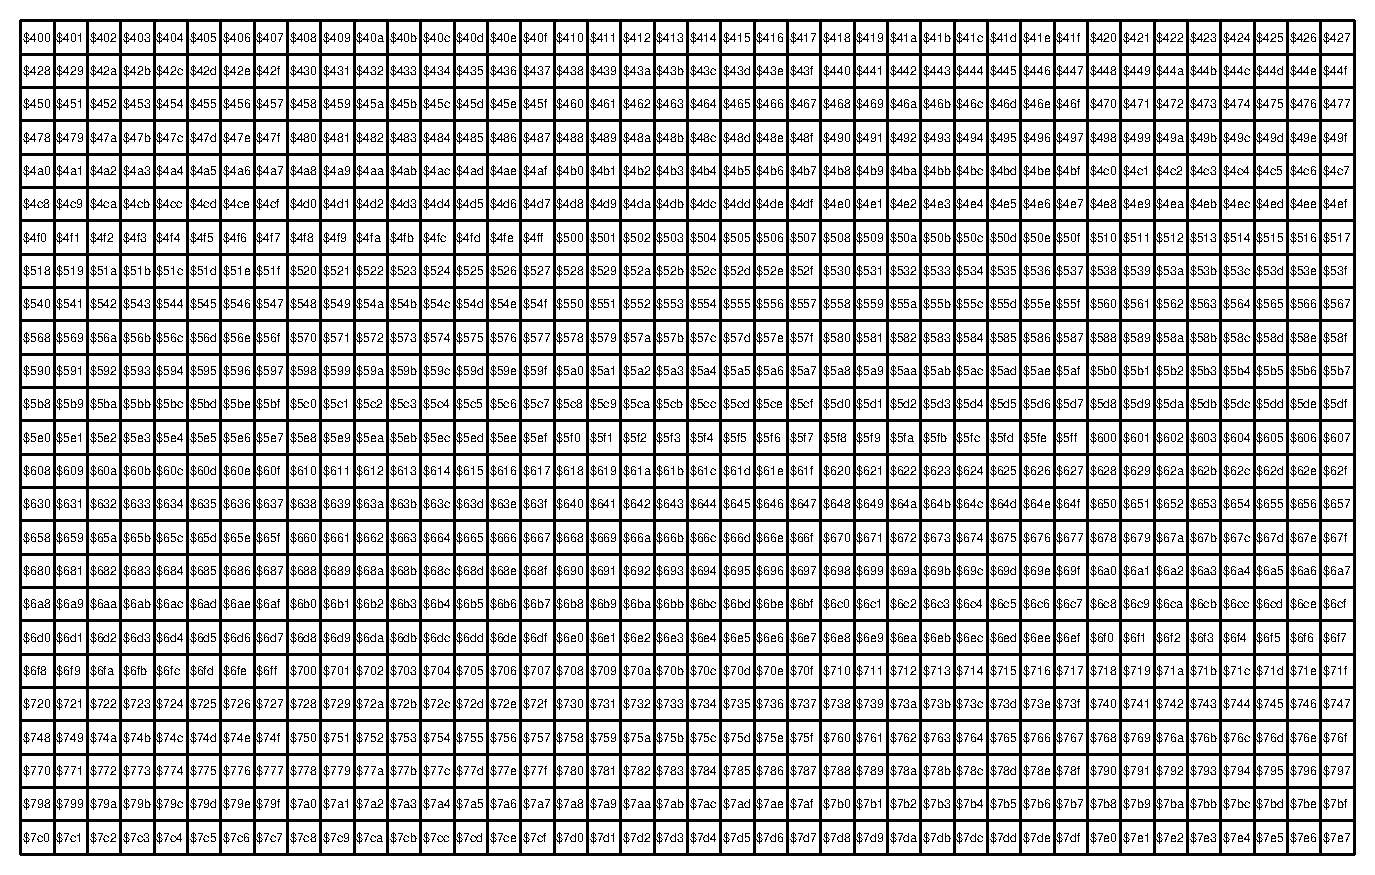
\includegraphics[width=\linewidth]{images/illustrations/screen-40x25-addresses.pdf}

That is, each character cell uses one byte of screen RAM, and the addresses increase smoothly, both within lines, and between lines.
Super-Extended Attribute Mode requires two bytes per character cell. So if you set \$D054 to \$05, for example, you will get screen addresses like this:

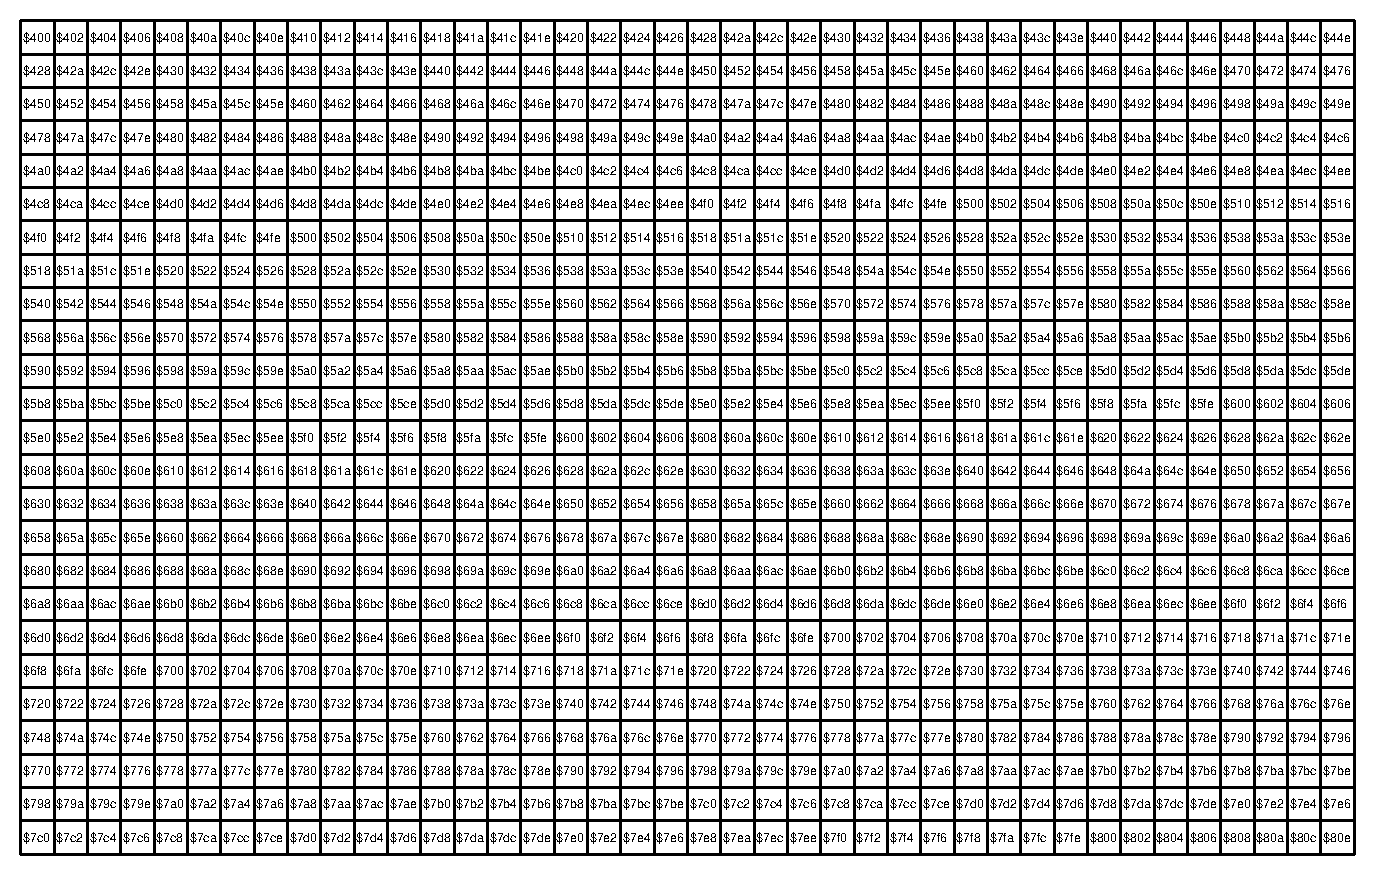
\includegraphics[width=\linewidth]{images/illustrations/screen-40x25-addresses16.pdf}

There are two things to notice in the above table: First, the address advances by two bytes for each character cell, because two bytes are required to define each character.  Second, the start address of each screen line still only advances by 40 (\$28 in hexadecimal). This isn't what we really want, because it means that half of the previous row will get displayed again on each current row.  This is fixed by setting the number of bytes to advance each screen row in \$D058 (LSB) and \$D059 (MSB). So in this case, we want to increase the number of bytes skipped each line from 40 bytes, to 80 bytes, which we can do by setting \$D058 to 80 (\$50 in hexadecimal), and \$D059 to 0.  This gives us a screen layout like this:

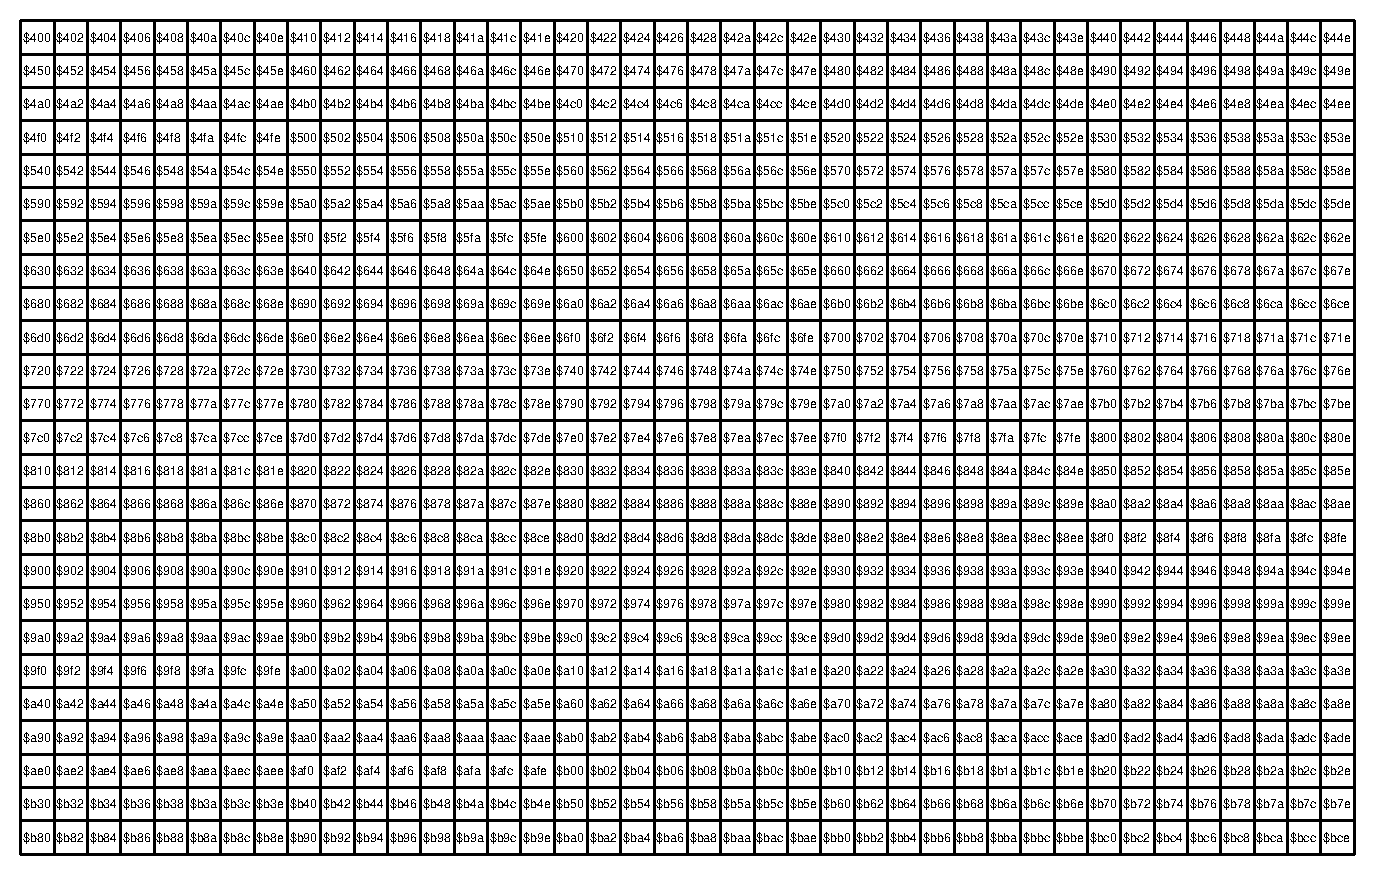
\includegraphics[width=\linewidth]{images/illustrations/screen-40x25-addresses16-80.pdf}

It is possible to use Super-Extended Attribute Mode from C65-mode, by setting the screen to 80 columns, as the C65 ROM sets up 2KB for both the screen RAM and colour RAM, and this automatically sets \$D058 and \$D059 to the correct value for 40$\times$2 = 80 bytes per screen line.  The user need only to treat each character pair as a single Super-Extended Attribute character, and to enable Super-Extended Attribute Mode, as described above.

Because pairs of colour RAM and screen RAM bytes are used to define each character, care must be taken to initialise and manipulate the screen.
A good approach is to set the text colour to black, because this is colour code 0, and then to fill the screen with @ characters, because that is
character code 0.  You can then have several ways to manipulate the screen.  You can use the normal PRINT command and carefully construct
strings that will put the correct values into each screen and colour byte pair. Another approach is to use the BANK and POKE commands to directly set the contents of the screen and colour RAM.

Managing a Super-Extended Attribute Mode screen in this way using BASIC 65 is of course rather a hack, and is only suggested as a relatively simple way to begin experimenting.  You will almost certainly want to quickly move to using custom screen handling code, most probably in assembly, to manipulate Super-Extended Attribute Mode screens, although this approach of using BASIC 65 can be quite powerful, by allowing use of existing screen scrolling and other manipulations.

XXX Example program

The following descriptions assume that you have implemented one of the methods described above to set the screen and colour RAM.

\subsection{Full-Colour (256 colours per character) Text Mode (FCM)}

In normal VIC-II/III text mode, one byte is used for each row of pixels in a character.  As a reminder for how those modes work, in
hi-res mode, each pixel is either the background or foreground colour, based on the state of one bit in the byte.  Multi-colour mode
uses two bits to select between four possible colours, but as there are still only 8 bits to describe each row of 8 pixels, each pair
of pixels has the same colour. The VIC-IV's full-colour text mode removes these limitations, and allows each pixel of a character to
be chosen from the 256 colour of either the primary or alternate palette bank, without sacrificing horizontal resolution.

To do this, each character now requires 64 bytes of data. The address of the data is 64 $\times$ the character number, regardless
of the character set address.
FCM should
normally be used with Super-Extended Attribute Mode (SEAM), so that more than 256 unique characters can be address. As SEAM allows
the selection of 8,192 unique characters, this allows FCM character data to be placed anywhere in the first 512KB of chip RAM (but
note that most models of the MEGA65 have only 384KB of chip RAM).

\subsection{Nibble-colour (16 colours per character) Text Mode (NCM)}

The Nibble-Colour Mode (NCM) for text is similar to Full-Colour Text Mode, except that each byte of data describes two
pixels using 4 bits each. This makes the NCM unique, because the characters will be 16 pixels wide, instead of the usual 8 pixels wide. This can be used to create colourful displays, without using as much memory as FCM, because fewer characters are required to cover the screen.  Unlike the VIC-II's MCM, this mode does not result in a loss of horizontal resolution.

In NCM the lower four bits of the pixel colour comes from the upper or lower four bits of the pixel data.  The upper four bits of the colour code come from the colour RAM data for the displayed character.  This makes it possible to use all palette entries in NCM, although the limitation of 16 colours per character remains.

A further advantage of NCM is that it uses fewer bus cycles per pixel than FCM, because fewer character data fetches need to occur per raster line.  Together with the reduced memory requirements, this makes NCM particularly useful for creating colourful multiple layers of graphics.  This allows the VIC-IV to display arcade style displays with more colours than many 16-bit computers.


XXX

\subsection{Alpha-Blending / Anti-Aliasing}

XXX

\subsection{Flipping Characters}

XXX

\subsection{Variable Width Fonts}

There are 4 bits that allow trimming pixels from the right edge of characters when they are displayed. This has the effect of making
characters narrower. This can be useful for making more attractive text displays, where narrow characters, such as ``i'' take less space than wider characters, such as ``m'', without having to use a bitmap display. This feature can be used to make it very efficient to display
such variable-width text displays -- both in terms of memory usage and processing time.

This feature can be combined with full-colour text mode, alpha blending mode and 4-bits per pixel mode to allow characters that consist of
15 levels of intensity between the background and foreground colour, and that are up to 16 pixels wide.  Further, the GOTO bit can be used to implement negative kerning, so that character pairs like A and T do not have excessive white space between them when printed adjacently. The prudent use of these features can result in highly impressive text display, similar to that on modern 32-bit and 64-bit systems, but that are still efficient enough to be implemented on a relatively constrained system such as the MEGA65. The ``MegaWAT!?'' presentation software for the MEGA65 uses several of these features to produce its attractive anti-aliased proportional text display on slides.

XXX MEGAWat!? screenshot

XXX Example program

\subsection{Raster Re-write Buffer}

If the GOTO bit is set for a character in Super-Extended Attribute Mode, instead of painting a character, the position on the raster is back-tracked (or advanced forward to) the
pixel position specified in the low 10 bits of the screen memory bytes.  If the vertical flip bit is set, then this has the alternate
meaning of preventing the background colour from being painted.  This combination can be used to print text material over the top of
other text material, providing a crude supplement to the 8 hardware sprites.  The amount of material is limited only by the raster
time of the VIC-IV. Some experimentation will be required to determine how much can be achieved in PAL and NTSC modes.

If the GOTO bit is set for a character, and the character width reduction bits are also set, they are interpretted as a Y offset to add to the character data address, but only in Full Colour Mode.  Setting Y=1 causes the character data to be fetched from 8 bytes later, i.e., the first row of character data will come from the address where the second row of character data would normally be fetched.  Similary for increased values the character data will be fetched from further character rows.  With careful arrangement of characters in memory, it is possible to use this feature to provide free vertical placement of soft sprites, without needing to copy the character data.

This ability to draw multiple layers of text and graphics is highly powerful. For example, it can be used to provide multiple overlapping
layers of separately scrollable graphics.  This gives many of the advantages of bitplane-based play-fields on other computers, such as the
Amiga, but without the disadvantages of bitplanes.

A good introduction to the Raster Re-write Buffer and its uses can be found in this video:

\url{https://www.youtube.com/watch?v=00bm5uBeBos&feature=youtu.be}

One important aspect of the RRB, is that the VIC-IV will display only the character data to the left of, and including, the last drawn character.  This means that if you use the GOTO token to overwrite multiple layers of graphics, you must either make sure that the last layer
reaches to the right-hand edge of the display, or you must include a GOTO token that moves the render position to the right-hand edge of the display.


XXX Example program

\section{Sprites}

\subsection{VIC-II/III Sprite Control}

The control of sprites for C64 / VIC-II/III compatibility is unchanged from the C64.  The only practical differences are very minor.
In particular the VIC-IV uses ring-buffer for each sprites data when rendering a raster. This means that a sprite can be displayed multiple times per raster line, thus potentially allowing for horizontal multiplexing.

\subsection{Extended Sprite Image Sets}

On the VIC-II and VIC-III, all sprites must draw their image data from a single 16KB region of memory at any point in time.
This limits the number of different sprite images to 256, because each sprite image occupies 64 bytes.  In practice, the same
16KB region must also contain either bitmap, text or bitplane data, considerably reducing the number of sprite images that
can be used at the same time.

The VIC-IV removes this limitation, by allowing sprite data to be placed anywhere in memory, although still on 64-byte
boundaries. This is done by setting the SPRPTR16 signal (bit 7, \$D06E, decimal 53358), which tells the VIC-IV to expect
two bytes per sprite pointer instead of one.  These addresses are then absolute addresses, and ignore the 16KB VIC-II
bank selection logic.  Thus 16 bytes are required instead of 8 bytes.  The list of pointers can also be placed anywhere
in memory by setting the SPRPTRADR (\$D06C -- \$D06D, 53356 -- 53357 decimal) and SPRPTRBNK signals (bits 0 -- 6, \$D06E, 53358 decimal).
This allows for sprite data to be located anywhere in the first 4MB of RAM, and the sprite pointer list to be located anywhere
in the first 8MB of RAM.  Note that typical installations of the VIC-IV have only 384KB of connected RAM, so these limitations are
of no practical effect. However, the upper bits of the SPRPTRBNK signal should be set to zero to avoid forward-compatibility
problems.

One reason for supporting more sprite images is that sprites on the VIC-IV can require more than one 64 byte image slot.
For example, enabling Extra-Wide Sprite Mode means that a sprite will require 8$\times$21 = 168 bytes, and will thus occupy
four VIC-II style 64 byte sprite image slots.  If variable height sprites are used, this can grow to as much as  8$\times$255 = 2,040 bytes per sprite.

\subsection{Variable Sprite Size}

Sprites can be one of three widths with the VIC-IV:

\begin{enumerate}
\item Normal VIC-II width (24 pixels wide).
\item Extra Wide, where 64 bits (8 bytes) of data are used per raster line, instead of the VIC-II's 24.
  This results in sprites that are 64 pixels wide, unless Full-Colour Sprite Mode is selected for a sprite,
  in which case the sprite will be 64 bits $\div$ 4 bits per pixel = 16 pixels wide.
\item Tiled mode, where the sprite is drawn repeatedly until the end of the raster line. \\
  Tiled mode should normally only be used with Extra Wide sprite mode, as the tiling always occurs using the full
64-bit sprite data. Thus if you use tiled mode with normal 24 pixel wide mono or multi-colour sprites, the tiling will treat each 2 and 2/3 rows of sprite data as a single row, resulting in garbled displays.
\end{enumerate}

To enable a sprite to be 64 pixels (or 16 pixels if in Full-Colour Sprite Mode), set the corresponding bit for the sprite in the SPRX64EN register at (\$D057, 53335 decimal).  Enabling Full Colour mode for a sprite implicitly enables extended width mode, causes these sprites to be 16 pixels wide.

Similarly, sprites can be various heights:  Sprites will be either the 21 pixels high of the VIC-II, or if the corresponding bit for the sprite is enabled in the SPRHGTEN signal (\$D055, 53333 decimal), then that sprite will be the number of pixels tall that is set in the SPRHGT
register (\$D056, 53334 decimal).

\subsection{Variable Sprite Resolution}

By default, sprites are the same resolution as on the VIC-II, i.e., each sprite pixel is two physical pixels wide and high.
However, sprites can be made to use the native resolution, where sprite pixels are one physical pixel wide and/or high.
This is achieved by setting the relevant bit for the sprite in the SPRENV400 (\$D076, 53366 decimal) registers to increase the
vertical resolution on a sprite-by-sprite basis.  The horizontal resolution for all sprites is either the normal VIC-II resolution, or if the SPR640 signal
is set (bit 4 of \$D054, 53332 decimal), then sprites will have the same horizontal resolution as the physical pixels of the display.

\subsection{Sprite Palette Bank}

The VIC-IV has four palette banks, compared with the single palette bank of the VIC-III.
The VIC-IV allows the selection of separate palette banks for bitmap/text graphics and for sprites.  This makes it easy to have
very colourful displays, where the sprites have different colours to the rest of the display, or to use palette animation to achieve
interesting visual effects in sprites, without disturbing the palette used by other elements of the display.

The sprite palette bank is selected by setting the SPRPALSEL signal in bits 2 and 3 of the register \$D070 (53360 decimal).
It is possible to set this to the same bank as the bitmap/text display, or to select a different palette bank.
Palette bank selection takes effect immediately.  Don't forget that to be able to modify a palette, you have to also bank it
to be the palette accessible via the palette bank registers at \$D100 -- \$D3FF by setting the MAPEDPAL signal in bits 6 and 7 of
\$D070.

\subsection{Full-Colour Sprite Mode}

In addition to monochrome and multi-colour modes, the VIC-IV supports a new full-colour sprite mode.  In this mode, four bits are used to
encode each sprite pixel.  However, unlike multi-colour mode where pairs of bits encode pairs of pixels, in full-colour mode the pixels
remain at their normal horizontal resolution.  The colour zero is considered transparent. If you wish to use black in a full-colour sprite, 
you must configure the palette bank that is selected for sprites so that one of the 15 colours for the specific sprite encodes black.

Full-colour sprite mode is selectable for each sprite by setting the appropriate bit in the SPR16EN register (\$D06B, 53355 decimal).

To enable the eight sprites to have 15 unique colours each, the sprite colour is drawn using the palette entry corresponding to:
$sprite number \times 16 + nibble value$, where $sprite number$ is the number of the sprite (from 0 to 7), and $nibble value$ is the value
of the half-byte that contains the sprite data for the pixel.  In addition, if bitplane mode is enabled for this sprite, then 128 is
added to the colour value, which makes it easy to switch between two colour schemes for a given sprite by changing only one bit in the
SPRBPMEN register.

Because Full-Colour Sprite Mode requires four bits per pixel, sprites will be only six pixels wide, unless Extra Wide Sprite Mode is enabled
for a sprite, in which case the sprite will be 16 pixels wide.  Tiled Mode also works with Full-Colour Sprite Mode, and will result in the
16 full-colour pixels of the sprite being repeated until the end of the raster line.

The following BASIC program draws a Full-Colour Sprite in either C64 or C65-mode:

\begin{screenoutput}
10 PRINT CHR$(147)
20 REM C65/C64-MODE DETECT
30 IF PEEK(53272) AND 32 THEN GOTO 100
40 POKE 53295,ASC("G"):POKE 53295,ASC("S")
100 REM SETUP SPRITE
110 AD=4096                         :REM $1000 SPRITE ADDR
120 TC=10                           :REM TRANSPARENT COLOUR
130 SPR=PEEK(53356)+PEEK(53357)*256 :REM GET SPRITE TABLE ADDRESS
140 POKE SPR,AD/64                  :REM SET SPRITE ADDRESS
150 FOR I=AD TO AD+168              :REM CLEAR SPRITE WITH TC
160 POKE I,TC+TC*16                 :REM ONE BYTE = 2 PIXEL
170 NEXT
180 POKE 53287,TC                   :REM SET TRANSPARENT COLOUR
190 POKE 53248,100                  :REM PUT SPRITE...
200 POKE 53249,100                  :REM ON SCREEN AT 100,100
210 POKE 53355,1                    :REM MAKE SPRITE 0 16-COLOUR
220 POKE 53335,1                    :REM MAKE SPRITE 0 USE 16X4-BITS
230 POKE 53269,1                    :REM ENABLE SPRITE 0
240 GOSUB 900                       :REM READ MULTI-COLOUR SPRITE
250 END

900 REM LOAD SPRITE FROM DATA
910 READ N$:IF N$="END" THEN RETURN
920 GOSUB 1000                      :REM DECODE LINE
930 GOTO 910

\end{screenoutput}

\begin{screenoutput}
1000 REM DECODE STRING OF NIBBLES IN N$ AT ADDRESS AD
1010 IF LEN(N$)<>16 THEN BEGIN:PRINT "ILLEGAL SPR DATA!":END:BEND
1020 FOR I=1 TO 16 STEP 2
1030 N=(ASC(MID$(N$,I,1))-ASC("@"))    :REM HIGH NYB
1040 IF N<0 THEN N=TC                  :REM . IS TRANSPARENT
1050 M=(ASC(MID$(N$,I+1,1))-ASC("@"))  :REM LOW NYB
1060 IF M<0 THEN M=TC                  :REM . IS TRANSPARENT
1070 POKE AD,(N AND 15)*16 + (M AND 15):REM SET 2 PIXELS
1080 AD=AD+1                           :REM ADVANCE AD
1090 NEXT I
1100 RETURN

1998 REM SPRITE DATA
1999 REM . = TRANSPARENT, @-O = COLOURS 0 TO 15
2000 DATA "..AAFF...HHCC..."
2010 DATA ".AAFF.....HHCC.."
2020 DATA "AAFF.......HHCC."
2030 DATA "AFF...@@@...HHC."
2040 DATA "FF..@@GGG@@..HH."
2050 DATA "..@@GGGGGGG@@..."
2060 DATA ".@GGGGGGGGGGG@.."
2070 DATA ".@GGGGGGGGGGG@.."
2080 DATA "@GGG@@GGG@@GGG@."
2090 DATA "@GG@GGGGGGG@GG@."
2100 DATA "@GGGGGGGGGGGGG@."
2110 DATA "@GGGGGBGBGGGGG@."
2120 DATA "@GGGBBBBBBBGGG@."
2130 DATA ".@GGGGBBBGGGG@.."
2140 DATA ".@GGGGGBGGGGG@.."
2150 DATA "..@@GGGGGGG@@..."
2160 DATA "II..@@GGG@@..KK."
2170 DATA "DII...@@@...KKE."
2180 DATA "DDII.......KKEE."
2190 DATA ".DDII.....KKEE.."
2200 DATA "..DDII...KKEE..."
2210 DATA "END"
\end{screenoutput}
\clearpage

\section{VIC-II / C64 Registers}

\input{regtable_VIC-II.C64}

\section{VIC-III / C65 Registers}

\input{regtable_VIC-III.C65}

\section{VIC-IV / MEGA65 Specific Registers}

\input{regtable_VIC-IV.MEGA65}
